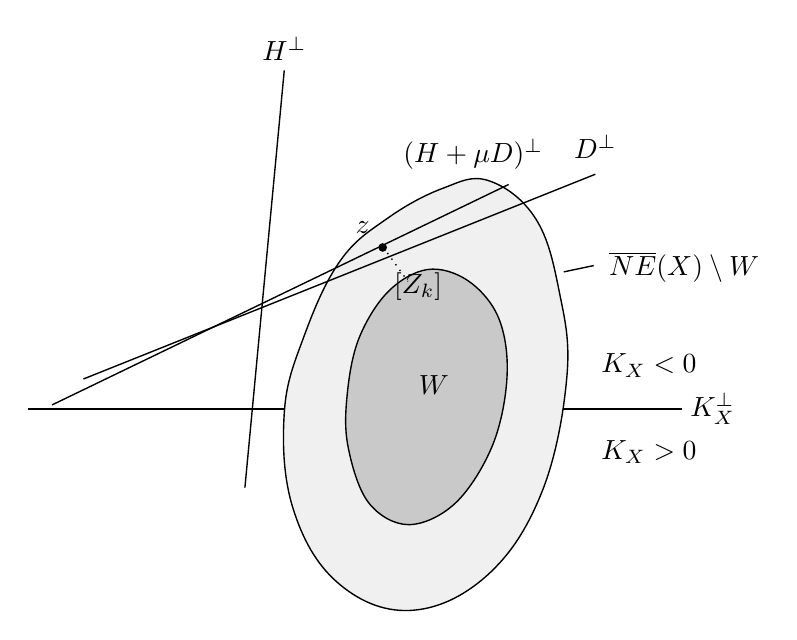
\begin{tikzpicture}[line width=0.5pt]
% 坐标轴
\draw (-2.20,0) -- (6.10,0);
\node[anchor=west] at (6.08,0.00) {$K_X^{\perp}$};
\node[anchor=west] at (4.95,0.55) {$K_X<0$};
\node[anchor=west] at (4.95,-0.55) {$K_X>0$};
% 外层区域 NE(X)\setminus W
\fill[gray!12] plot[smooth cycle, tension=0.65] coordinates
 {(1.05,-0.05) (1.30,0.92) (1.76,1.88) (2.36,2.42) (3.06,2.80)
  (3.64,2.90) (4.24,2.42) (4.54,1.50) (4.64,0.42) (4.32,-1.06)
  (3.62,-2.12) (2.64,-2.56) (1.72,-2.20) (1.16,-1.26)};
\draw plot[smooth cycle, tension=0.65] coordinates
 {(1.05,-0.05) (1.30,0.92) (1.76,1.88) (2.36,2.42) (3.06,2.80)
  (3.64,2.90) (4.24,2.42) (4.54,1.50) (4.64,0.42) (4.32,-1.06)
  (3.62,-2.12) (2.64,-2.56) (1.72,-2.20) (1.16,-1.26)};
% 内层区域 W
\fill[gray!42] plot[smooth cycle, tension=0.60] coordinates
 {(1.85,0.19) (2.00,0.90) (2.37,1.49) (2.87,1.77) (3.38,1.63)
  (3.77,1.16) (3.88,0.43) (3.70,-0.45) (3.23,-1.19) (2.63,-1.47)
  (2.12,-1.19) (1.86,-0.48)};
\draw plot[smooth cycle, tension=0.60] coordinates
 {(1.85,0.19) (2.00,0.90) (2.37,1.49) (2.87,1.77) (3.38,1.63)
  (3.77,1.16) (3.88,0.43) (3.70,-0.45) (3.23,-1.19) (2.63,-1.47)
  (2.12,-1.19) (1.86,-0.48)};
% 三条直线（共点于 P）
\coordinate (P) at (0.80,1.30);
\draw (1.05,4.30) -- (0.55,-1.00);
\draw (3.90,2.85) -- (-1.90,0.05);
\draw (5.00,2.98) -- (-1.50,0.38);
\node[above] at (1.05,4.30) {$H^{\perp}$};
\node[above] at (3.45,2.92) {$(H+\mu D)^{\perp}$};
\node[above] at (5.00,3.05) {$D^{\perp}$};
% 点 z 与 [Z_k]
\fill (2.30,2.05) circle (0.055);
\node[above left] at (2.26,2.10) {$z$};
\node at (2.75,1.55) {$[Z_k]$};
\draw[dotted] (2.36,1.98) -- (2.62,1.62);
% 区域标注
\node at (2.95,0.30) {$W$};
\node[anchor=west] (outs) at (5.05,1.80) {$\overline{NE}(X)\setminus W$};
\draw (4.98,1.82) -- (4.60,1.74);
\end{tikzpicture}
